
\section{Test set up}\label{section:testSetUp}
The measurement for this LIDAr was done by measuring the distance between  the sensor and an target, both rotating and while standstill (static) for to acquire the necessary data. Figure \ref{fig:testSetUp} describes how the test set up was done.
%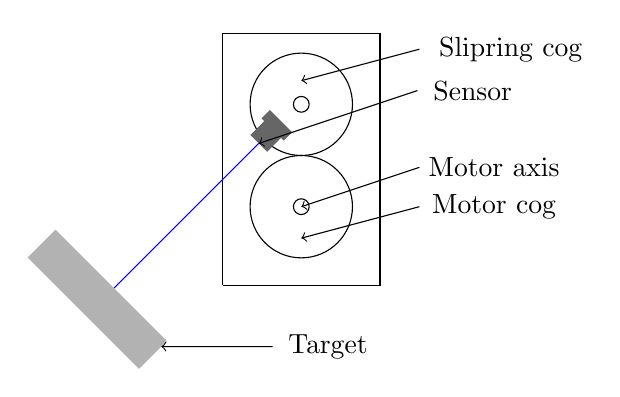
\begin{tikzpicture}[xscale=0.5, yscale=0.5]
\draw (0,0) -- (4,0) -- (4,6.4) -- (0,6.4) -- (0,0); %outre box
\draw (2,2) circle (1.3); %cog for motor
\draw (2,2) circle (0.2); % axis for motor
\draw (2,4.6) circle (1.3); %cog for slipring
\draw (2,4.6) circle (0.2); %axis for silp ring

%Sensor of the top cog
\fill[black!60!white, rotate=-45] (-2.3,4.0) rectangle (-1.5,3.7);
\fill[black!60!white, rotate=-45] (-2.2,3.2) rectangle (-1.6,3.8);
%beeam
\draw[blue, rotate=-45] (-1.9,3.2) -- (-1.9,-2);
%target
\fill[black!30!white, rotate=-45] (-4,-2) rectangle (0,-3);

%arrows
\draw[->, rotate=-45] (0,7)node[xshift=20] {Sensor} -- (-1.9,3.2);
\draw[->] (5,3)node[xshift=27] {Motor axis} -- (2.0,2.0) ;% motor axis
\draw[->] (5,2)node[xshift=27] {Motor cog} -- (2.0,1.2);% motor cog
\draw[->] (5,6)node[xshift=33] {Slipring cog} -- (2.0,5.2);% lidar cog
\draw[->, rotate=-45] (2,-0.2)node[xshift=20] {Target} -- (-0.0,-2.2);

\end{tikzpicture}
\begin{figure}[ht]
    \centering
   %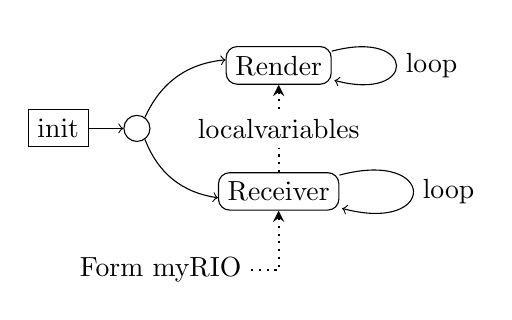
\begin{tikzpicture}
\tikzstyle{rounded} = [rectangle, rounded corners , minimum width=3mm, minimum height=1mm,text centered, draw=black]
\tikzstyle{round}=[circle, minimum width=0mm,draw=black]
\tikzstyle{square} = [rectangle, minimum width=1mm, draw=black]
\tikzstyle{empty}=[]

\usetikzlibrary{shapes.geometric, arrows}
\tikzstyle{arrow} = [thick,->,>=stealth]
\tikzstyle{dottarrow} = [thick, dotted,->,>=stealth]
\tikzstyle{dottline} = [thick, dotted,-,>=stealth]
\tikzstyle{noarrow}=[thick,-=,=stealth]

%nodes
\node (init) [square] {init};
\node (loop) [round, right of=init]{};
\node (render)[rounded, right of=loop, xshift=8mm, yshift=8mm ] {Render};
\node (rezive) [rounded, right of=loop, xshift=8mm, yshift=-8mm] {Receiver};
\node (datain) [empty, below of=rezive, xshift=-15mm]{Form myRIO};
\node (shared) [empty, below of=render, yshift=2mm]{localvariables};


%lines
%(Startnode)  edge [bend arrow]       node[text pos]  {text}          (target);
\path[->] 
(init) 		edge 								node[left]		{}			(loop)
(loop)		edge[bend left] 					node[left]		{}			(render)
(loop)		edge[bend right]					node[left]		{}			(rezive)
(render) 	edge[loop right]					node[right]		{loop}			(render)
(rezive) 	edge[loop right]					node[right]		{loop}			(rezive)
;
\draw [dottarrow] (datain) -| (rezive);
%\draw [dottarrow] (rezive) -- (render);
\draw [dottline] (rezive) -- (shared);
\draw [dottarrow] (shared) -- (render);

\end{tikzpicture}
   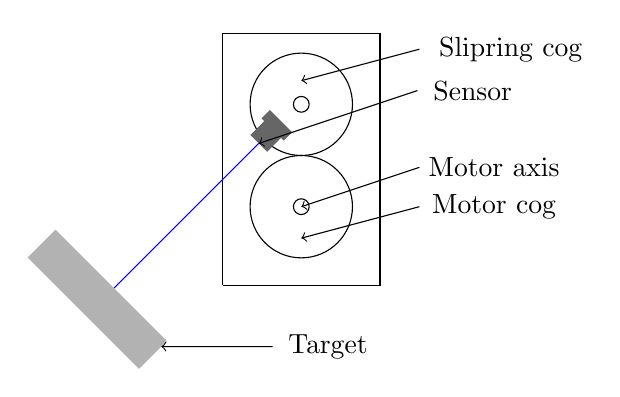
\begin{tikzpicture}[xscale=0.5, yscale=0.5]
\draw (0,0) -- (4,0) -- (4,6.4) -- (0,6.4) -- (0,0); %outre box
\draw (2,2) circle (1.3); %cog for motor
\draw (2,2) circle (0.2); % axis for motor
\draw (2,4.6) circle (1.3); %cog for slipring
\draw (2,4.6) circle (0.2); %axis for silp ring

%Sensor of the top cog
\fill[black!60!white, rotate=-45] (-2.3,4.0) rectangle (-1.5,3.7);
\fill[black!60!white, rotate=-45] (-2.2,3.2) rectangle (-1.6,3.8);
%beeam
\draw[blue, rotate=-45] (-1.9,3.2) -- (-1.9,-2);
%target
\fill[black!30!white, rotate=-45] (-4,-2) rectangle (0,-3);

%arrows
\draw[->, rotate=-45] (0,7)node[xshift=20] {Sensor} -- (-1.9,3.2);
\draw[->] (5,3)node[xshift=27] {Motor axis} -- (2.0,2.0) ;% motor axis
\draw[->] (5,2)node[xshift=27] {Motor cog} -- (2.0,1.2);% motor cog
\draw[->] (5,6)node[xshift=33] {Slipring cog} -- (2.0,5.2);% lidar cog
\draw[->, rotate=-45] (2,-0.2)node[xshift=20] {Target} -- (-0.0,-2.2);

\end{tikzpicture}
  \caption{The LIDAR had the construction with an slip ring to allow free passage of the cable without being twinned. Therefore it used 2 3D printed cogs to transfer the rotation from the motor to the sensor. The lower circle describe the cog that was connected to the motor whiles the top one with the sensor describe the cog that had an slip ring in it. There are also an target to the bottom left, how ever the distance is not up to scale hear for spacing reason.}
  \label{fig:testSetUp}
\end{figure}

\section{Measurement and test results}\label{secition:results}
The measurements that was taken for this report was done both while the motor was rotating and standing still (static). And are represented as polar plots and histogram of the distance.

\subsection{Smallest detectable object}\label{subsection:mesurment-smalest}
The smallest object that the sensor can detect is dependent on zise of the object, speed of the LIDAR and distance between the LIDAR and the object.

In our test we tested with an round object that had a diameter of $6mm$. 
After a series of test the conclusion was that it could see the object in between $113mm$ and $300mm$ when the delay was $40ms$ in between each step.
If the step delay adjusted down to $1ms$ the LIDAR was still able to detect it sometimes and the range decreased to below $230mm$.


\subsection{Minimum speed}\label{subsetion:mesurmen-miniSpeed}
The minimum speed was also dependent on in with direction the object travelled in relation to the LIDAR. 
Al test was done with an one meter long wooden plank that was hanging from a string so it could be easy manipulated.
When the object approached the LIDAR that was rotating with an delay of $1.5ms$ against the LIDARs beam the measurement showed that the object wasent detecteble if the object moved faster then $1m/s$. 
The other direction gave the result $0.4m/s$ dependent a bit of the initial position.

\subsection{Different objects}\label{subsection:mesurment-difObj}
The test that was preformed was if the LIDAR could see an transparent acrylic box.
And the data suggested it wasn't any big difference between the box and the solid object. 
Highly reflective material was only captured when it was almost orgogonal to the object.

\subsection{The sensors accuracy}\label{subsubsection:accuracy}
Data for the sensors accuracy was obtained by using the function described earlier in section \ref{subsubsection:comphistogram}. The data that was captured is as shown in figure \ref{fig:test-hist}.

\begin{figure}[ht]
    \centering
   %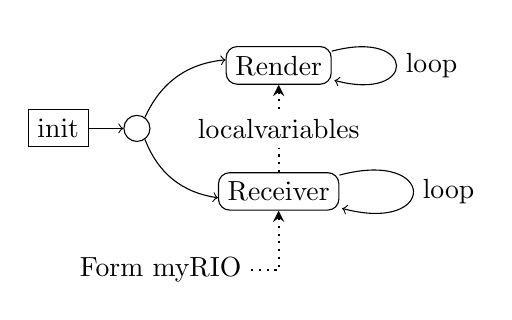
\begin{tikzpicture}
\tikzstyle{rounded} = [rectangle, rounded corners , minimum width=3mm, minimum height=1mm,text centered, draw=black]
\tikzstyle{round}=[circle, minimum width=0mm,draw=black]
\tikzstyle{square} = [rectangle, minimum width=1mm, draw=black]
\tikzstyle{empty}=[]

\usetikzlibrary{shapes.geometric, arrows}
\tikzstyle{arrow} = [thick,->,>=stealth]
\tikzstyle{dottarrow} = [thick, dotted,->,>=stealth]
\tikzstyle{dottline} = [thick, dotted,-,>=stealth]
\tikzstyle{noarrow}=[thick,-=,=stealth]

%nodes
\node (init) [square] {init};
\node (loop) [round, right of=init]{};
\node (render)[rounded, right of=loop, xshift=8mm, yshift=8mm ] {Render};
\node (rezive) [rounded, right of=loop, xshift=8mm, yshift=-8mm] {Receiver};
\node (datain) [empty, below of=rezive, xshift=-15mm]{Form myRIO};
\node (shared) [empty, below of=render, yshift=2mm]{localvariables};


%lines
%(Startnode)  edge [bend arrow]       node[text pos]  {text}          (target);
\path[->] 
(init) 		edge 								node[left]		{}			(loop)
(loop)		edge[bend left] 					node[left]		{}			(render)
(loop)		edge[bend right]					node[left]		{}			(rezive)
(render) 	edge[loop right]					node[right]		{loop}			(render)
(rezive) 	edge[loop right]					node[right]		{loop}			(rezive)
;
\draw [dottarrow] (datain) -| (rezive);
%\draw [dottarrow] (rezive) -- (render);
\draw [dottline] (rezive) -- (shared);
\draw [dottarrow] (shared) -- (render);

\end{tikzpicture}
        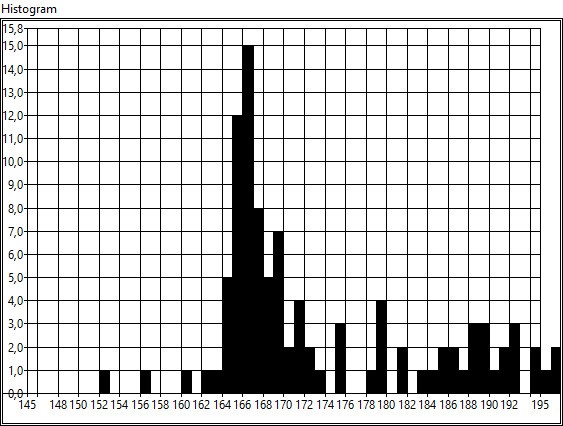
\includegraphics[scale=0.2] {./mesurment/data/Expected_170,0__Mean_176,02__Distrubution_13,567648_Rotating_1ms}
       % 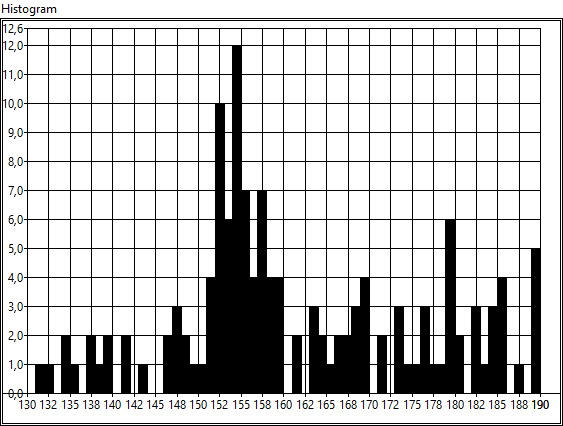
\includegraphics[scale=0.2] {./mesurment/data/Expected_160,0__Mean_161,13__Distrubution_14,311767_Rotating_5ms}
       % \\
       % 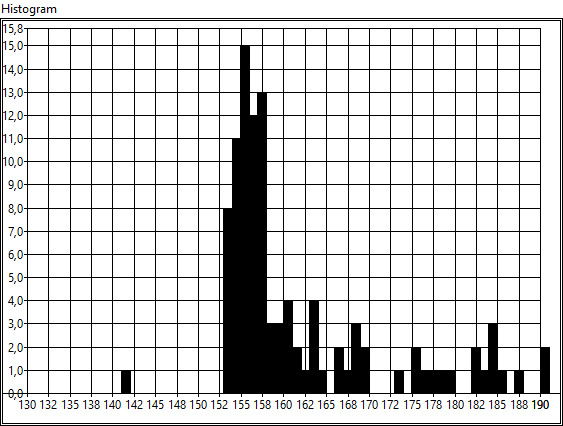
\includegraphics[scale=0.2] {./mesurment/data/Expected_160,0__Mean_161,29__Distrubution_10,066412_Rotating_10ms}
        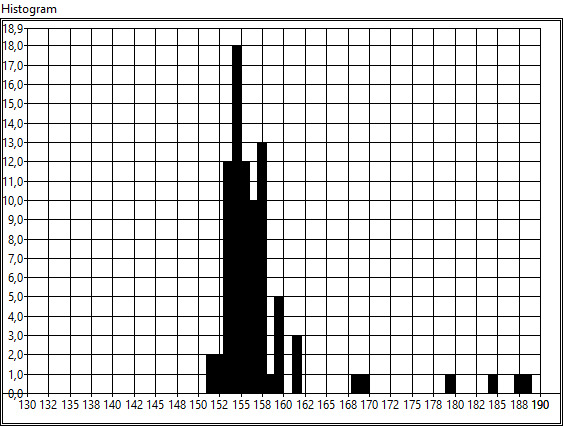
\includegraphics[scale=0.2] {./mesurment/data/Expected_160,0__Mean_156,97__Distrubution_6,850402_Rotating_40ms}
  %\caption{The delay between each step. Top left:1ms, Top right: 5ms, Bottom left:10ms, Bottom right: 40ms. As the data shows the accuracy of the sensor is worse in between 5 and 10ms.}
        \caption{A rotating LIDAR. Left exacted object at $ \mu=170mm $  for the rotational delay of $1ms$ the distribution was $13.6mm&. Right $ \mu=160mm$ for the delay of $40ms$ and gave the distrbution of $6.9mm$.}
  \label{fig:test-hist}
\end{figure}

%But locking only at the data form the distribution formula don't actually say anything as can be shown in figure \ref{table:rotating}.
%\begin{figure}
    \begin{center}
        \small
        \begin{tabular}{ l | l | l | r| }
            Expected&Mean&Distrubution&Delay\\
            \hline
            160&  160,5& 12,139055 & 1ms\\
            170&  176,0& 13,567648 & 1ms\\
            160&  161,1& 14,311767 & 5ms\\
            188&  183,5& 14,132543 & 5ms\\
            160&  161,2& 10,066412 & 10ms\\
            188&  183,4& 7,866309  & 15ms\\
            190&  184,7& 3,113610  & 30ms\\
            160&  156,9& 6,850402  & 40ms\\
            190&  186,0& 3,205185  & 50ms\\
            160&  156,0& 5,257015  & 50ms
        \end{tabular}
    \end{center}
    \caption{When the lidar moves the the accuracy goes down while the speed goes up. However from this table alone the observer can not derive to any real conclution because of the random noise in figure \ref{fig:test-hist}.}
    \label{table:rotating}
\end{figure}

%However it is interesting to compare the results in the figure \ref{table:rotating} with an static measurement where the sensor don't rotate and that can be found in figure \ref{table:static}.
%\begin{figure}
    \begin{center}
        \small
        \begin{tabular}{ l | l | l }
            Expected&Mean&Distribution\\
        \hline
            120& 117,68 & 0,537\\
            190& 186,46 & 1,057\\
            201& 202,17 & 7,497\\
            242& 242,70 & 1,418\\
            300& 303,84 & 2,078\\
            350& 344,56 & 37,53\\
            400& 386,12 & 25,08
        \end{tabular}
    \end{center}
    \caption{When the sensor is stationary the accuracy goes up but only up to a certain distance then the sensor data begins to deviate again.}
    \label{table:static}
\end{figure}


\subsection{LIDAR measurements}\label{subsection:lidarmeaurment}
The rotating sensor for the LIDAR have as shown in the chapter \ref{subsubsection:mesure} loses its accuracy the faster the sensor moves.
%That can be shown in the figure \ref{fig:lidar-images} and therefore as the speed increases the noise also increases, but it is absolutely worst between 5 and 10ms because the construction shakers more at those speeds causing the sensor to make some random readings.

\begin{figure}[ht]
    \centering
   %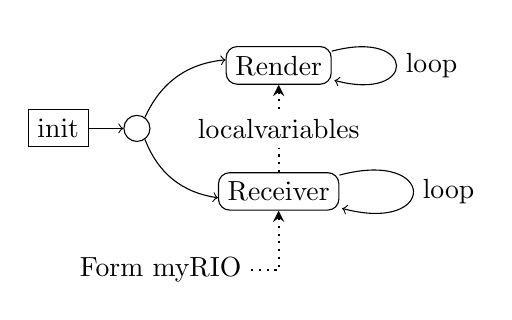
\begin{tikzpicture}
\tikzstyle{rounded} = [rectangle, rounded corners , minimum width=3mm, minimum height=1mm,text centered, draw=black]
\tikzstyle{round}=[circle, minimum width=0mm,draw=black]
\tikzstyle{square} = [rectangle, minimum width=1mm, draw=black]
\tikzstyle{empty}=[]

\usetikzlibrary{shapes.geometric, arrows}
\tikzstyle{arrow} = [thick,->,>=stealth]
\tikzstyle{dottarrow} = [thick, dotted,->,>=stealth]
\tikzstyle{dottline} = [thick, dotted,-,>=stealth]
\tikzstyle{noarrow}=[thick,-=,=stealth]

%nodes
\node (init) [square] {init};
\node (loop) [round, right of=init]{};
\node (render)[rounded, right of=loop, xshift=8mm, yshift=8mm ] {Render};
\node (rezive) [rounded, right of=loop, xshift=8mm, yshift=-8mm] {Receiver};
\node (datain) [empty, below of=rezive, xshift=-15mm]{Form myRIO};
\node (shared) [empty, below of=render, yshift=2mm]{localvariables};


%lines
%(Startnode)  edge [bend arrow]       node[text pos]  {text}          (target);
\path[->] 
(init) 		edge 								node[left]		{}			(loop)
(loop)		edge[bend left] 					node[left]		{}			(render)
(loop)		edge[bend right]					node[left]		{}			(rezive)
(render) 	edge[loop right]					node[right]		{loop}			(render)
(rezive) 	edge[loop right]					node[right]		{loop}			(rezive)
;
\draw [dottarrow] (datain) -| (rezive);
%\draw [dottarrow] (rezive) -- (render);
\draw [dottline] (rezive) -- (shared);
\draw [dottarrow] (shared) -- (render);

\end{tikzpicture}
        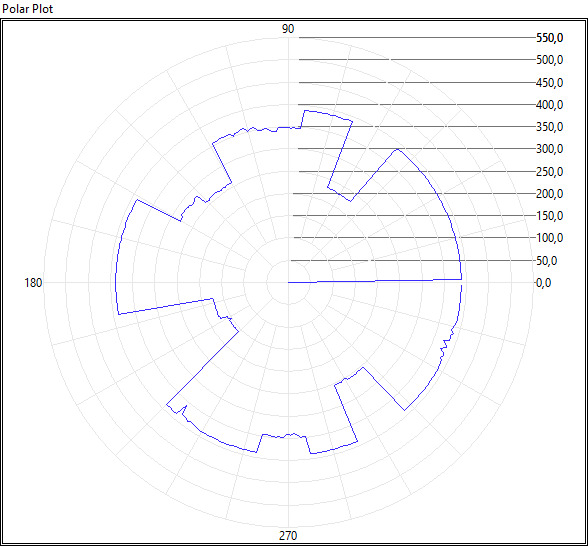
\includegraphics[scale=0.2]{./mesurment/data/Lidar_1ms_9_oclock_detection}
        %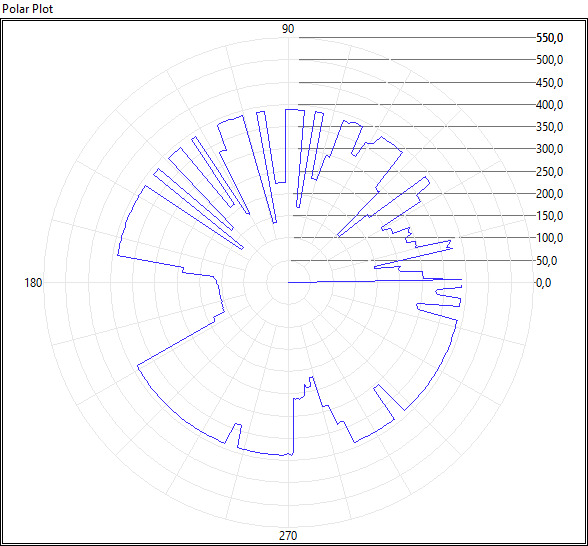
\includegraphics[scale=0.2]{./mesurment/data/Lidar_10ms_9_oclock_detection}\\
        %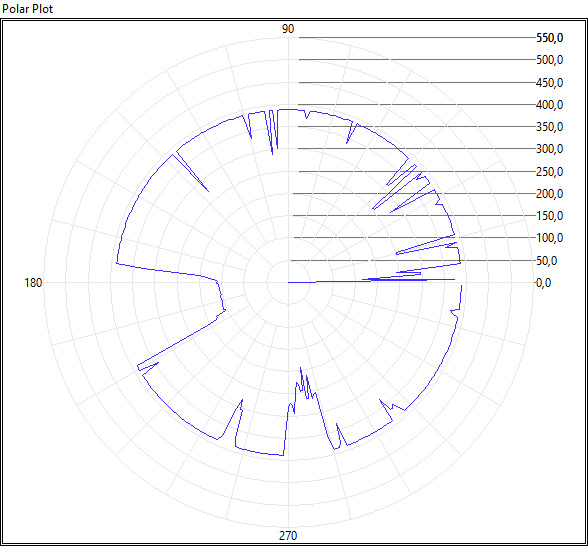
\includegraphics[scale=0.2]{./mesurment/data/Lidar_30ms_9_oclock_detection}
        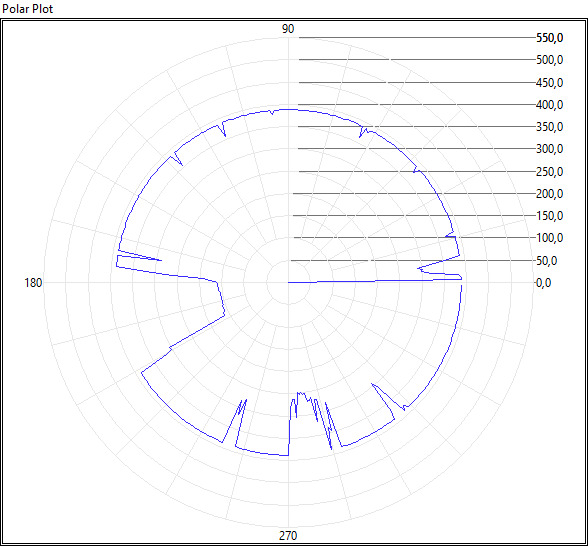
\includegraphics[scale=0.2]{./mesurment/data/Lidar_40ms_9_oclock_detection}
 %\caption{}
  %\caption{In this figure the only object that should be there is the object at $(x=-1, y=0)$ the rest is ghost except perhaps the one in the bottom because its the motor shaft that is going throw the cog and interferes with the sensor.}
  \caption{ The render LIIDAR output with an object detected at the left, note that the detection in the bottom is mostlikly a detection of the motor axis.   }
  \label{fig:lidar-images}
\end{figure}

